\documentclass{Trade_template}
\usepackage[a4paper,pdftex]{geometry}                                                                           % A4paper margins
\setlength{\oddsidemargin}{5mm}                                                                                         % Remove 'twosided' indentation
\setlength{\evensidemargin}{5mm}
\usepackage[protrusion=true,expansion=true]{microtype}  
\usepackage{amsmath,amsfonts,amsthm,amssymb}
\usepackage{graphicx}
\usepackage{parallel,enumitem}
\usepackage{amssymb}
\usepackage{float}
\usepackage{rotating}
\usepackage{amsmath, bm}
\usepackage{amsfonts}
\usepackage[T1]{fontenc}
\usepackage[polish,english]{babel}
\usepackage[utf8]{inputenc}
\usepackage{lmodern}
\usepackage{array}
\usepackage{etoolbox}
\usepackage{hyperref}
\usepackage{algorithm2e}
\usepackage[noend]{algpseudocode}
\usepackage{listings}
\usepackage[usenames,dvipsnames]{xcolor}
\usepackage{booktabs}
\usepackage{caption} 
\captionsetup[table]{skip=10pt}
\captionsetup[algorithm2e]{skip=10pt}
\usepackage{booktabs,caption,fixltx2e}
\usepackage[para,online,flushleft]{threeparttable}
\usepackage{adjustbox}
\usepackage{lscape}
\usepackage[round]{natbib}
\bibliographystyle{plainnat}
\usepackage{nameref}
\usepackage{tabularx}
\usepackage{subcaption}

\hypersetup{pdfstartview={XYZ null null 1.00}}

\hypersetup{
    colorlinks,
    linkcolor={red!50!black},
    citecolor={blue!50!black},
    urlcolor={blue!80!black}
}

\numberwithin{equation}{section}
\newcolumntype{Y}{>{\centering\arraybackslash}X}
\newcolumntype{L}{>{\centering\arraybackslash}m{2.5cm}}
\newcolumntype{M}{>{\centering\arraybackslash}m{3.5cm}}

\lstset{ %
  language=python,                     % the language of the code
  basicstyle=\footnotesize,       % the size of the fonts that are used for the code
  numbers=left,                   % where to put the line-numbers
  numberstyle=\tiny\color{gray},  % the style that is used for the line-numbers
  stepnumber=1,                   % the step between two line-numbers. If it's 1, each line
                                  % will be numbered
  numbersep=5pt,                  % how far the line-numbers are from the code
  backgroundcolor=\color{white},  % choose the background color. You must add \usepackage{color}
  showspaces=false,               % show spaces adding particular underscores
  showstringspaces=false,         % underline spaces within strings
  showtabs=false,                 % show tabs within strings adding particular underscores
  frame=single,                   % adds a frame around the code
  rulecolor=\color{black},        % if not set, the frame-color may be changed on line-breaks within not-black text (e.g. commens (green here))
  tabsize=2,                      % sets default tabsize to 2 spaces
  captionpos=b,                   % sets the caption-position to bottom
  breaklines=true,                % sets automatic line breaking
  breakatwhitespace=false,        % sets if automatic breaks should only happen at whitespace
  title=\lstname,                 % show the filename of files included with \lstinputlisting;
                                  % also try caption instead of title
  keywordstyle=\color{blue},      % keyword style
  commentstyle=\color{ForestGreen},   % comment style
  stringstyle=\color{Orchid},      % string literal style
  escapeinside={\%*}{*)},         % if you want to add a comment within your code
  morekeywords={*,...}            % if you want to add more keywords to the set
} 

\lstset{ %
  language=R,                     % the language of the code
  basicstyle=\footnotesize,       % the size of the fonts that are used for the code
  numbers=left,                   % where to put the line-numbers
  numberstyle=\tiny\color{gray},  % the style that is used for the line-numbers
  stepnumber=1,                   % the step between two line-numbers. If it's 1, each line
                                  % will be numbered
  numbersep=5pt,                  % how far the line-numbers are from the code
  backgroundcolor=\color{white},  % choose the background color. You must add \usepackage{color}
  showspaces=false,               % show spaces adding particular underscores
  showstringspaces=false,         % underline spaces within strings
  showtabs=false,                 % show tabs within strings adding particular underscores
  frame=single,                   % adds a frame around the code
  rulecolor=\color{black},        % if not set, the frame-color may be changed on line-breaks within not-black text (e.g. commens (green here))
  tabsize=2,                      % sets default tabsize to 2 spaces
  captionpos=b,                   % sets the caption-position to bottom
  breaklines=true,                % sets automatic line breaking
  breakatwhitespace=false,        % sets if automatic breaks should only happen at whitespace
  title=\lstname,                 % show the filename of files included with \lstinputlisting;
                                  % also try caption instead of title
  keywordstyle=\color{blue},      % keyword style
  commentstyle=\color{ForestGreen},   % comment style
  stringstyle=\color{Orchid},      % string literal style
  escapeinside={\%*}{*)},         % if you want to add a comment within your code
  morekeywords={*,...}            % if you want to add more keywords to the set
} 


\author{Michał Miktus, Mateusz Szmidt}

\nralbumu{}

\title{Machine learning approach \\
to trade flows estimation}

\kierunek{Analysis and Policy in Economics}

\opiekun{Pablo Winant Ph. D.\\
  Paris School of Economics\\
  }

\date{March 2019}

\newtheorem{theorem}{Theorem}
\newtheorem{corollary}{Corollary}[theorem]
\newtheorem{lemma}{Lemma}
\newtheorem{mydef}{Definition}

\begin{document}
\maketitle

\tableofcontents
\listoffigures
\listoftables
%\listofalgorithms


\chapter*{Introduction} \label{Introduction}
\addcontentsline{toc}{chapter}{Introduction}

Since the pioneer work of \citet{tinbergen1962analysis}, the gravity equations has been widely implemented in the estimation of bilateral trade flows. The fundamental insight that the volume of trade between two countries is proportional to the product of an index of their economic sizes diminished by the measures of “trade resistance” between them has shaped the empirical specifications mainly due to the surprisingly good fit to the majority of data sets of both regional, as well as international trade flows. Over time the \citet{tinbergen1962analysis} approach has been modified and enhanced, not to mention the supplementary theoretical underpinnings such as additional measures of trade resistance in spite of the classical ones (geographic distance, a dummy for common borders or dummies for Commonwealth memberships) or better estimation methods, allowing for the inclusion of zero-trade flows in the framework. 

The following paper aims to implement the modern machine learning algorithms in the framework of gravity modeling in order to predict the bilateral trade flows. Machine learning can be viewed as an application of artificial intelligence (AI) which provides systems the ability to automatically learn and improve from experience without being explicitly programmed. In other words, machine learning focuses on the development of computer programs that can access data and use it learn for themselves, without human intervention or assistance, and adjust actions accordingly. The latest advancements in machine learning allowed to effortlessly identify patterns in data and use them to automatically make predictions or decisions. To the authors' best knowledge, the following paper is the first try in implementing the above-mentioned framework to the trade policy analysis.

In addition, due to the familiarity of both authors to the Polish trade environment, the Poland trade relations has been chosen as a workhorse illustration. Obtained results prove that a neural network approach can be viewed as a grievous challenger to the classical estimation methods, such as Poisson Pseudo-Maximum Likelihood models or ordinary fixed panel data estimators.

The paper is organized as follows: the first chapter consists of the brief literature review, including the common gravity models and the estimation techniques, followed by the data characterization. Next sections provide a detailed description of the neural network approach enhanced by the hyper-parameters tuning and outline the main results. The paper is completed with the concluding remarks with potential extensions, references and appendices with codes in R and Python.

\chapter{Literature review}

The traditional gravity model was developed in the 1960s to explain factory-to-consumer trade (\citet{tinbergen1962analysis}). The above-mentioned concept was at the heart of the first clear microfoundations of the gravity equation – the seminal \citet{anderson1979theoretical}, proposing a theoretical explanation of the gravity equation based on constant elasticity of substitution preferences of nations producing a single differentiated product. In parallel, the monopolistic competition versions were introduced (\citet{krugman1980scale}, \citet{bergstrand1985gravity}), followed by the work of \citet{anderson2003gravity}, expanding appropriate econometric techniques and introducing the microeconomic framework to the previously promoted monopolistic competition. Subsequent theoretical refinements have further focused on showing that the gravity equation can be derived from trade models with heterogeneous firms (\citet{helpman2008estimating}).

Simultaneously, the estimation techniques were progressing, starting from the basic least square estimator and its correspondent panel data version, meaning the fixed effect estimator. The endogeneity issues guided to the establishment of instrumental variables and two step least squares methodologies in the gravity models framework. Therefore, the Poisson Pseudo-Maximum Likelihood (henceforth PPML) model, introduced by \citet{santos2006ppml}, as well as zero-inflated models were proposed in order to solve the mentioned problems. Over the years, they became the flagship framework for the bilateral trade flows estimation with some dominance of PPML, mainly due to its statistical properties such as robustness to different forms of heteroskedasticity.

However, the aforementioned advantage was often criticized over the years, not to mention \citet{martin2008gravity} who admitted that PPML estimator is in fact less biased than formerly used methods, but not necessarily fully unbiased. This view was further supported by \citet{martinez2013gravity} who compared it within a family of GLS models, arguing that the appropriate estimation method should be chosen with a greater caution. Consequently, authors attempt to propose a machine learning neural network algorithm as a potential competitor to the Poisson Pseudo-Maximum Likelihood estimator in the context of bilateral trade flows.


\chapter{Data exploration}

For the first part of the data, namely the set of explanatory variables, the CEPII statistics were used, resulting in annual data of 60 variables at the cross country level. Then, using 3 digit ISO codes the dataset was joined with the trade flows information. Nevertheless, in contrary to the first, fully available online dataset, in order to obtain data on flows from Comtrade database, a data scrapper needed to be created. The authors expanded and modified the scrapping function delivered by Comtrade which in the end allowed to bypass all the limitations build into basic API and optimize the time of data scrapping. The exact code can be found in \nameref{Appendix A}. 

The final variables used in the calculations, along with their descriptions, are presented in the table \nameref{Desc}, while the basic summary statistics are illustrated in the table \nameref{Stats}.

\newpage 

\begin{sidewaystable}[ph!]
    \centering
    \caption[Summary statistics]{Summary statistics}
    \label{Stats}
\tiny{
\begin{tabularx}{\textwidth}{@{} L *{12}{Y}  @{}}
\toprule
Variable & count & unique & top & freq & mean & std & min & 25\% & 50\% & 75\% & max & cova  \\ \midrule
gatt\_o & 4060.00 & NaN & NaN & NaN & 1.00 & 0.00 & 1.00 & 1.00 & 1.00 & 1.00 & 1.00 & 0.00 \\
area\_o & 4060.00 & NaN & NaN & NaN & 312685.00 & 0.00 & 312685.00 & 312685.00 & 312685.00 & 312685.00 & 312685.00 & 0.00 \\
yr & 4060.00 & NaN & NaN & NaN & 2004.49 & 6.31 & 1994.00 & 1999.00 & 2005.00 & 2010.00 & 2015.00 & 0.00 \\
pop\_o & 4060.00 & NaN & NaN & NaN & 38.33 & 0.22 & 38.00 & 38.15 & 38.23 & 38.54 & 38.66 & 0.01 \\
gdp\_o & 4060.00 & NaN & NaN & NaN & 3.19e+11 & 1.55e+11 & 1.09e+11" & 1.72e+11" & 3.04e+11 & 4.77e+11 & 5.45e+11 & 0.48 \\
gdpcap\_o & 4060.00 & NaN & NaN & NaN & 8339.74 & 4052.41 & 2819.70 & 4483.24 & 7976.12 & 12554.55 & 14341.86 & 0.49 \\
gatt\_d & 4060.00 & NaN & NaN & NaN & 0.75 & 0.43 & 0.00 & 1.00 & 1.00 & 1.00 & 1.00 & 0.57 \\
distw & 4060.00 & NaN & NaN & NaN & 6140.89 & 3899.61 & 387.07 & 2603.11 & 5845.77 & 8583.18 & 17653.91 & 0.64 \\
eu\_o & 4060.00 & NaN & NaN & NaN & 0.55 & 0.50 & 0.00 & 0.00 & 1.00 & 1.00 & 1.00 & 0.91 \\
tdiff & 4060.00 & NaN & NaN & NaN & 3.38 & 3.12 & 0.00 & 1.00 & 2.00 & 6.00 & 12.00 & 0.92 \\
comrelig & 4060.00 & NaN & NaN & NaN & 0.25 & 0.28 & 0.00 & 0.01 & 0.11 & 0.45 & 0.79 & 1.15 \\
gdpcap\_d & 4060.00 & NaN & NaN & NaN & 10410.33 & 16066.97 & 64.81 & 864.06 & 3223.29 & 13299.54 & 116612.88 & 1.54 \\
gsp\_o\_d & 4060.00 & NaN & NaN & NaN & 0.24 & 0.43 & 0.00 & 0.00 & 0.00 & 0.00 & 1.00 & 1.80 \\
fta\_wto & 4060.00 & NaN & NaN & NaN & 0.23 & 0.42 & 0.00 & 0.00 & 0.00 & 0.00 & 1.00 & 1.84 \\
eu\_to\_acp & 4060.00 & NaN & NaN & NaN & 0.21 & 0.40 & 0.00 & 0.00 & 0.00 & 0.00 & 1.00 & 1.96 \\
comleg\_pretrans & 4060.00 & NaN & NaN & NaN & 0.17 & 0.38 & 0.00 & 0.00 & 0.00 & 0.00 & 1.00 & 2.20 \\
transition\_legalchange & 4060.00 & NaN & NaN & NaN & 0.13 & 0.34 & 0.00 & 0.00 & 0.00 & 0.00 & 1.00 & 2.55 \\
area\_d & 4060.00 & NaN & NaN & NaN & 719321.80 & 1956801.49 & 25.00 & 25713.00 & 119902.00 & 547244.00 & 17075400.00 & 2.72 \\
eu\_d & 4060.00 & NaN & NaN & NaN & 0.11 & 0.32 & 0.00 & 0.00 & 0.00 & 0.00 & 1.00 & 2.81 \\
comleg\_posttrans & 4060.00 & NaN & NaN & NaN & 0.10 & 0.30 & 0.00 & 0.00 & 0.00 & 0.00 & 1.00 & 2.96 \\
pop\_d & 4060.00 & NaN & NaN & NaN & 34.23 & 129.66 & 0.01 & 1.69 & 6.66 & 21.70 & 1371.22 & 3.79 \\
gdp\_d & 4060.00 & NaN & NaN & NaN & 2.64e+11 & 1.13e+12 & 1.09e+07 & 3.16e+09 & 1.46e+10 & 1.04e+11 & 1.80e+13 & 4.30 \\
Trade\_value\_total & 4060.00 & NaN & NaN & NaN & 1.12e+09 & 5.30e+09 & 0.00 & 1.52e+06 & 2.34e+07 & 2.35e+08 & 1.03e+11 & 4.74 \\
contig & 4060.00 & NaN & NaN & NaN & 0.04 & 0.19 & 0.00 & 0.00 & 0.00 & 0.00 & 1.00 & 5.04 \\
sibling & 4060.00 & NaN & NaN & NaN & 0.03 & 0.16 & 0.00 & 0.00 & 0.00 & 0.00 & 1.00 & 6.02 \\
colony & 4060.00 & NaN & NaN & NaN & 0.01 & 0.07 & 0.00 & 0.00 & 0.00 & 0.00 & 1.00 & 13.55 \\
col\_fr & 4060.00 & NaN & NaN & NaN & 0.01 & 0.07 & 0.00 & 0.00 & 0.00 & 0.00 & 1.00 & 13.55 \\
heg\_d & 4060.00 & NaN & NaN & NaN & 0.01 & 0.07 & 0.00 & 0.00 & 0.00 & 0.00 & 1.00 & 13.55 \\
rt3ISO & 4060.00 & 1 & POL & 4060 & NaN & NaN & NaN & NaN & NaN & NaN & NaN & NaN \\
pt3ISO & 4060.00 & 190 & ARE & 22 & NaN & NaN & NaN & NaN & NaN & NaN & NaN & NaN \\
iso2\_o & 4060.00 & 1 & PL & 4060 & NaN & NaN & NaN & NaN & NaN & NaN & NaN & NaN \\
iso2\_d & 4060.00 & 190 & BZ & 22 & NaN & NaN & NaN & NaN & NaN & NaN & NaN & NaN \\
comlang\_off & 4060.00 & NaN & NaN & NaN & 0.00 & 0.00 & 0.00 & 0.00 & 0.00 & 0.00 & 0.00 & NaN \\
comlang\_ethno & 4060.00 & NaN & NaN & NaN & 0.00 & 0.00 & 0.00 & 0.00 & 0.00 & 0.00 & 0.00 & NaN \\
comcol & 4060.00 & NaN & NaN & NaN & 0.00 & 0.00 & 0.00 & 0.00 & 0.00 & 0.00 & 0.00 & NaN \\
col45 & 4060.00 & NaN & NaN & NaN & 0.00 & 0.00 & 0.00 & 0.00 & 0.00 & 0.00 & 0.00 & NaN \\
heg\_o & 4060.00 & NaN & NaN & NaN & 0.00 & 0.00 & 0.00 & 0.00 & 0.00 & 0.00 & 0.00 & NaN \\
col\_to & 4060.00 & NaN & NaN & NaN & 0.00 & 0.00 & 0.00 & 0.00 & 0.00 & 0.00 & 0.00 & NaN \\
curcol & 4060.00 & NaN & NaN & NaN & 0.00 & 0.00 & 0.00 & 0.00 & 0.00 & 0.00 & 0.00 & NaN \\
cursib & 4060.00 & NaN & NaN & NaN & 0.00 & 0.00 & 0.00 & 0.00 & 0.00 & 0.00 & 0.00 & NaN \\
comcur & 4060.00 & NaN & NaN & NaN & 0.00 & 0.00 & 0.00 & 0.00 & 0.00 & 0.00 & 0.00 & NaN \\
legold\_o & 4060.00 & 1 & so & 4060 & NaN & NaN & NaN & NaN & NaN & NaN & NaN & NaN \\
legold\_d & 4060.00 & 5 & fr & 1759 & NaN & NaN & NaN & NaN & NaN & NaN & NaN & NaN \\
legnew\_o & 4060.00 & 1 & ge & 4060 & NaN & NaN & NaN & NaN & NaN & NaN & NaN & NaN \\
legnew\_d & 4060.00 & 5 & fr & 2153 & NaN & NaN & NaN & NaN & NaN & NaN & NaN & NaN \\
acp\_to\_eu & 4060.00 & NaN & NaN & NaN & 0.00 & 0.00 & 0.00 & 0.00 & 0.00 & 0.00 & 0.00 & NaN \\
gsp\_d\_d & 4060.00 & NaN & NaN & NaN & 0.00 & 0.00 & 0.00 & 0.00 & 0.00 & 0.00 & 0.00 & NaN \\
flaggsp\_o\_d & 4060.00 & 3 & no gsp recorded in Rose & 3099 & NaN & NaN & NaN & NaN & NaN & NaN & NaN & NaN \\
flaggsp\_d\_d & 4060.00 & 1 & no gsp recorded in Rose & 4060 & NaN & NaN & NaN & NaN & NaN & NaN & NaN & NaN \\ \bottomrule
\end{tabularx}}
\caption*{\tiny{Where the columns denote respectively the variables described, the number of observations, the amount of unique values, the most frequent value (for categorical variables), the frequency of the most frequent value, the mean, the standard deviation, the minimum value, the first quantile, the median, the third quantile, the maximum value and finally the coefficient of variation.}}
\end{sidewaystable}

\newpage

\begin{table}[H]
\centering
\caption[Variables and their description]{Variables and their description} \label{Desc}
\small{
\begin{tabularx}{\textwidth}{@{} M X  @{}}
\toprule
Variable & Description \\ \midrule
yr & Year \\ rt3ISO & Standard ISO code for reporting country (three letters) \\
pt3ISO & Standard ISO code for partner country (three letters) \\
contig & Dummy for contiguity \\
heg\_d & Dummy if parter country is current or former hegemon of origin \\
col\_fr & Dummy for reporting and partner countries colonial relationship post 1945 \\
colony & Dummy for reporting and partner countries ever in colonial relationship \\
sibling & Dummy for reporting and partner countries ever in sibling relationship i.e. two colonies of the same empire \\
comleg\_pretrans & Dummy if reporting and partner countries share common legal origins before transition \\
comleg\_posttrans & Dummy if reporting and partner countries share common legal origins after transition \\
transition\_legalchange & Dummy if common legal origin changed since transition \\
legold\_d & Legal system of partner country before transition. This variable takes the values: fr for French, ge for German, sc for Scandinavian, so for Socialist and uk for British legal origin \\
legnew\_d & Legal system of partner country after transition. This variable takes the values: fr for French, ge for German, sc for Scandinavian, so for Socialist and uk for British legal origin \\
gatt\_d & Dummy if partner country is GATT/WTO member \\
fta\_wto & Dummy for Regional Trade Agreement \\
eu\_to\_acp & Dummy for ACP country exporting to EC/EU member \\
gsp\_o\_d & Dummy if origin is donator in Generalized System of Preferences (GSP) \\
flaggsp\_o\_d & Report changes in Roses data on \textless{}gsp\_o\_d\textgreater{}. No gsp recorded in Rose; Data directly from Rose; Changes in data from Rose; Assumption that gsp continues after 1999 \\
eu\_o & Dummy if reporting country a member of the European Union \\
eu\_d & Dummy if partner country a member of the European Union \\
Trade\_value\_total & Total value of trade between reporting and partner countries \\
distw & Weighted bilateral distance between reporting and partner countries in kilometer (population weighted) \\
pop\_o & Population of reporting country total in million \\
pop\_d & Population of partner country total in million \\
gdp\_o & GDP of reporting country (current US\$) \\
gdp\_d & GDP of partner country (current US\$) \\
gdpcap\_o & GDP per capita of reporting country (current US\$) \\
gdpcap\_d & GDP per capita of partner country (current US\$) \\
area\_d & Area of partner country in sq. kilometers \\
tdiff & Time difference between reporting and partner countries in number of hours. For countries which stretch over more than  one  time  zone   the  respective  time  zone  is generated via the mean of all its time zones (for instance: Russia, Canada, USA) \\
comrelig & Religious proximity (\citet{disdier2007je}) is an index calculated by adding the products of the shares of Catholics, Protestants and Muslims in the exporting and importing countries. It is bounded between 0 and 1 and is maximum if the country pair has a religion which (1) comprises a vast majority of the population and (2) is the same in both countries. \\ \bottomrule
\end{tabularx}}
\end{table}

\newpage

Furthermore, due to the fact that the authors concentrated their attention on the trade flows of Poland with its partner, the following graphs demonstrate that Poland mainly trades with Unites States, China and Europe.

\begin{figure}[H]
        \centering
        \begin{subfigure}[b]{0.475\textwidth}
            \centering
            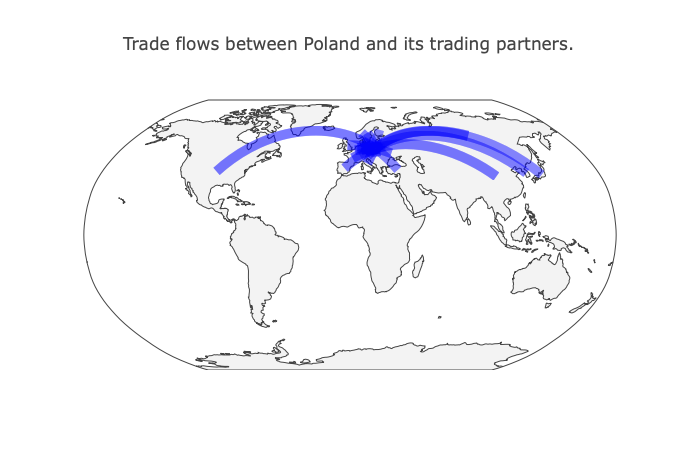
\includegraphics[width=\textwidth]{Flows}
\caption[Trade flows between Poland and its world trading partners]{Trade flows between Poland and its world trading partners}
        \end{subfigure}
        \hfill
        \begin{subfigure}[b]{0.475\textwidth}  
            \centering 
            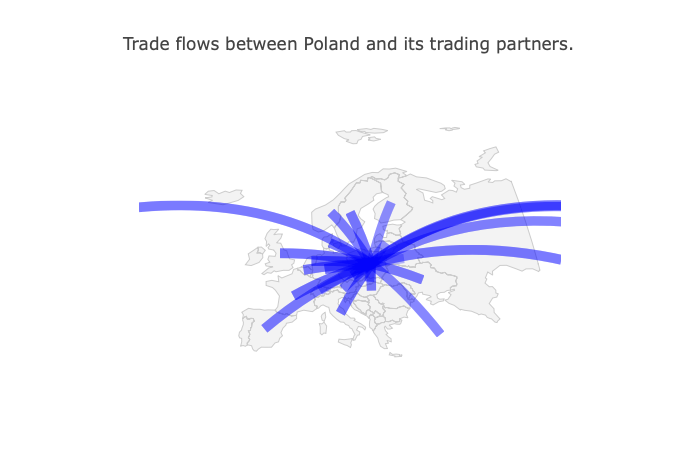
\includegraphics[width=\textwidth]{Flows_Europe}
\caption[Trade flows between Poland and its European trading partners]{Trade flows between Poland and its European trading partners}
        \end{subfigure}
\caption[Trade flows between Poland and its trading partners]{Trade flows between Poland and its trading partners}
\end{figure}

Moreover, the histogram of standarized trade flows of Poland from 1994 to 2015 certifies that there is a relatively large group of countries with which Poland is not involved in trading relations. 

\begin{figure}[H]
\centering
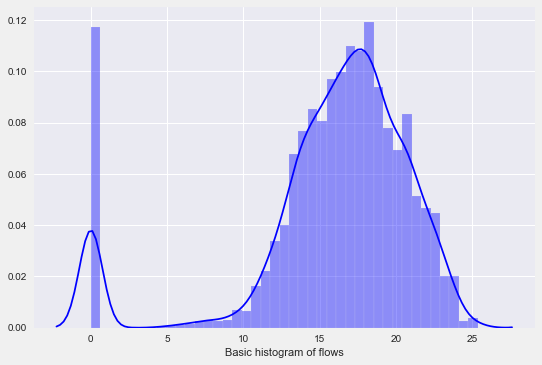
\includegraphics[width=0.9\textwidth]{Histogram_of_flows_over_the_history}
\caption[Histogram of flows over the history]{Histogram of flows over the history (overall)}
\end{figure} 

\newpage

The aforementioned fact it complemented with the histograms in specific years: 1994, 2000, 2009 and 2015. However, it can be noticed that the amount of trading partners was gradually increasing over time.

\begin{figure}[H]
        \centering
        \begin{subfigure}[b]{0.475\textwidth}
            \centering
            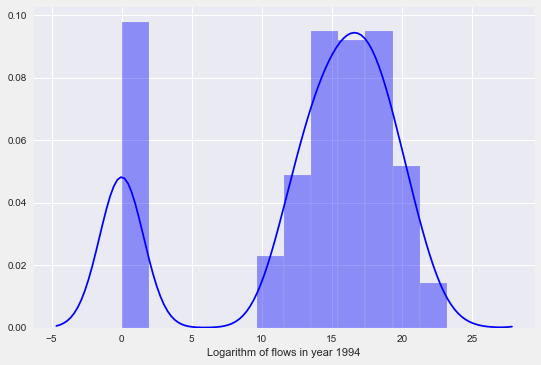
\includegraphics[width=\textwidth]{Histogram1994}
            \caption[Histogram of flows in 1994]%
            {{\small Histogram of flows in 1994}}    
            \label{hist1994}
        \end{subfigure}
        \hfill
        \begin{subfigure}[b]{0.475\textwidth}  
            \centering 
            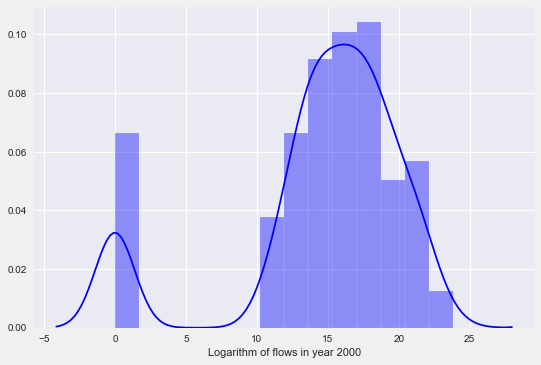
\includegraphics[width=\textwidth]{Histogram2000}
             \caption[Histogram of flows in 2000]%
            {{\small Histogram of flows in 2000}}    
            \label{hist2000}
        \end{subfigure}
        \vskip\baselineskip
        \begin{subfigure}[b]{0.475\textwidth}   
            \centering 
            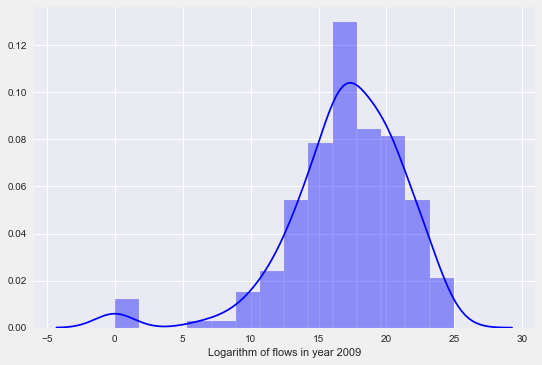
\includegraphics[width=\textwidth]{Histogram2009}
             \caption[Histogram of flows in 2009]%
            {{\small Histogram of flows in 2009}}    
            \label{hist2009}
        \end{subfigure}
        \quad
        \begin{subfigure}[b]{0.475\textwidth}   
            \centering 
            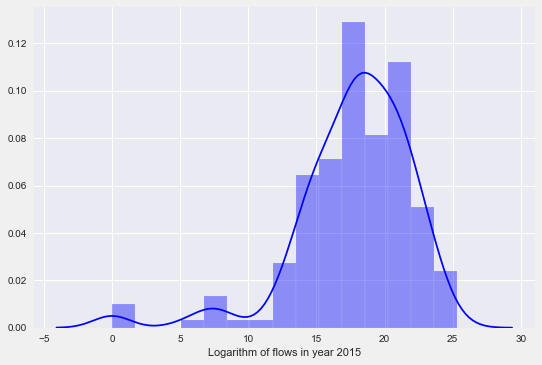
\includegraphics[width=\textwidth]{Histogram2015}
             \caption[Histogram of flows in 2015]%
            {{\small Histogram of flows in 2015}}    
            \label{hist2015}
        \end{subfigure}
        \caption[Histogram of flows in specific years]
        {\small Histogram of flows in specific years} 
        \label{hist_specific}
    \end{figure}

Finally, as the main interest of the following paper is the gravity model, the relations between total trade value, distance and partner country's GDP (standarized) are demonstrated in the pairplots graphs.

\newpage

\begin{figure}[H]
\centering
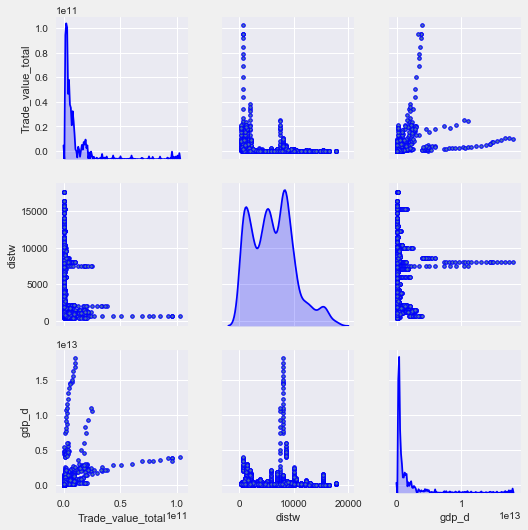
\includegraphics[width=0.9\textwidth]{Pairplots}
\caption[Pairplots]{Pairplots between total trade value, distance and partner country's GDP (standarized)}
\end{figure} 

Accordingly to the intuition, the value of trade is lower for the more distanced countries, while on contrary it seems to be positively correlated with the trading country's gross domestic product, which can be regarded as the proxy for the nation's size.

\chapter{Neural network approach}

The neural networks approach is a statistical framework allowing to find complex patterns of relations in the data. The intuition behind the above-mentioned concept is often compared to the way of how human nerve system functions. In a nutshell, it can be characterized as follows - in the first phase the external signal is received by receptors and transferred to the set of neurons. Then, during further stages, it is iteratively processed and passed to next set of neurons until the signal is finally decoded. The structure of the neural network model similarly compounds of 3 elements: the input layer of independent variables, set of "hidden layers” and finally the output layer with calculated results of a model. Given the structure, in each phase besides the last one, the values of nodes from former layer are affinely transformed and then nonlinear function in performed in order to obtain the values for each node of a new layer. The calculations are repeated until the last phase when the final value is accessed through a nonlinear function of affine product of nodes from previous layers. The aforementioned process, starting from an input data and aiming to compute the output, is called the \textit{forward propagation} and can be seen as a function of coefficients coined within every single affine transformation taking place between all neighbouring layers.

As a result, the estimated trade flows from the neural network approach rely on finding the appropriate values of parameters under arbitrary selected structure of a model. Thus in the first stage, the values of the coefficients are randomly assigned and then the forward propagation is performed. Next, based on model’s output and true values of the observable dependent variable, the arbitrary chosen loss function is calculated. It has to be underlined that due to the fact that the generated output is a result of forward propagation, the loss function can be also defined as a function of the same parameters. It allows to compute a derivative with respect to them and in the end, to recalibrate their values – such a process is called  \textit{backward propagation} and it is iteratively repeated together with forward propagation to minimize the loss function, optimizing the values of parameters. 

Although the intuition and general process behind the estimation of neural network model were presented above, a plethora of aspects referred to depends on arbitrary chosen structure or so called \textit{architecture of a model}. Therefore, some choices implemented in the final, best suited to the data architecture of the model need to be elaborated.

Firstly, a number of hidden layers intuitively allows to approximate any continuous function more carefully, nevertheless adding any next layer is computationally costly. The charge born is strictly related to another element of a model’s structure, namely the number of neurons in each layer. It has to be emphasised that the above-mentioned amount can be different depending on a layer but again bigger number directly translates into higher cost. Consequently, to take advantage of computer architecture and to optimize processing time, a power of 2 neurons in each layer were implemented, as suggested in the literature.

It has been already mentioned that each node is in fact defined as a function of the values of neurons from the former layer. It is thus beneficial to remark that it can be enforced that a node from hidden layer is a function of only a subset of nodes from a former one. Depending on the problem such an idea might be intuitive, not to mention the picture recognition, but it does not seem to be relevant in trade flows case. What is more, during the learning process such an exclusion of particular nodes may appear anyway, when the weights in affine transformations are relatively close to zero. Thus, the network with nodes being functions of all previous ones will be considered.

Moreover, the nonlinear transformation of a product of former nodes has to be defined. In the neural network framework, it is often called \textit{an activation function}, aiming to activate the particular neuron on a hidden layer and assign to it some positive value when the particular pattern within a former nodes is observed. In a neural network literature, a particular set of functions can be observed, which by construction allows the model to be trained faster due to computational advantage while deriving derivatives and which satisfy the basic intuition behind activation. The most common ones are presented below.

\begin{figure}[H]
\centering
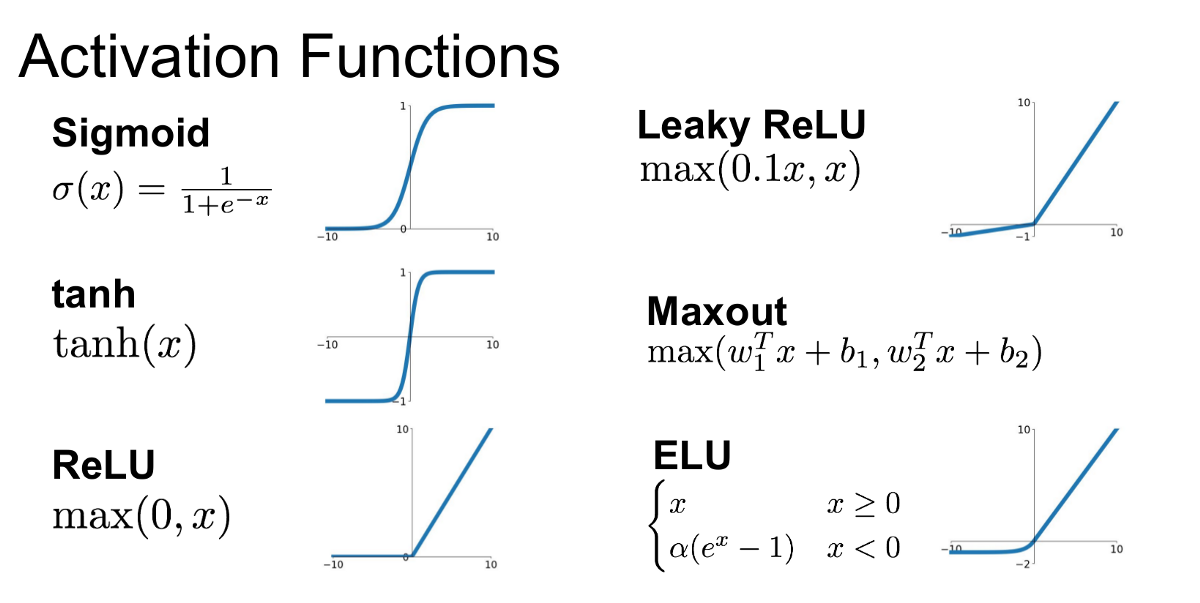
\includegraphics[width=0.9\textwidth]{Activation}
\caption[Activation functions]{Activation functions\footnotemark}
\end{figure} 

\footnotetext{Source: \url{https://bit.ly/2uh7NyV}}

The actually implemented in the end are sigmoid and relu. The first one was especially popular in the past, while the second one gained the popularity recently, outperforming the former with respect to the computational time.

At this stage, the part of hyper-parameters of models’ structure directly connected to the forward propagation was covered. As far as the backward propagation choices are concerned, a loss function given the generated output has to be chosen. In the paper, the mean squared error was selected to validate the output. Moreover, in order to prevent the problem of overfitting, the regularization was implemented. The role of the aforementioned concept is simply to penalize the actual loss function of the model so that increase of the coefficients to some extent negatively affects the loss function. The value of a hyper-parameter of a penalty function identifies the size of marginal increase in a loss function alone to be compensated by the penalty. 

Another regularization approach which can be implemented simultaneously is dropout. It serves to omit a fraction of randomly chosen nodes (along with their connections) on each layer while performing both forward and backward propagation. Thus, it enforces iterative deactivation of different neurons which diminish the pace of convergence but also stanches from overfitting the model. Nevertheless, it may simultaneously negatively influence the convergence, therefore a maximum number of iterations, in neural network framework called \textit{epochs}, has to be specified. Choice of its value always brings a trade-off between a computational time and optimality of solution. One way (actually implemented in the paper) of meeting halfway is to set a threshold for marginal increase in loss function, ending the learning process sooner if the condition is fulfilled.

In fact, it is a learning process itself which determines the final performance of neural network framework. To fully define it, few more elements of a model’s structure have to be recalled. As mentioned before, the estimation is based on calculating numerous derivatives with respect to all the parameters, according to the chain-rule, which in the end determines for a given set of parameters’ values a point-gradient. However, as the neural networks tend to be defined over an enormous parameter space, the straightforward calculation of a gradient might be a complex task itself. Therefore, different optimization algorithms were implemented. The first one is Stochastic Gradient Decent (SGD), which calculates new iteration of parameters according to the specified learning rate, which is in turn another hyper-parameter of the model, defining the convergence speed. However, in standard SGD the learning rate is not scalable and it poorly handles updating the parameters of high variance. To deal with it, the second method is proposed, namely the Adam optimizer, which becomes gradually common recently. It allows to adjust the specified learning rate for each parameter and is often more efficient. Lastly, to speed up the whole process the hyper-parameter called batch size can be defined. The model chooses a subsample in a size of batch and performs an iteration using only selected observations. Therefore, it allows to train the model each time on different observation set and reduces the complexity of the whole process.

At this stage all the elements of model architecture are defined, allowing to implement the neural network on the presented grid of hyper-parameters and proceed with an estimation, with exact codes included in \nameref{Appendix B}.

\chapter{Results}

As far as the main outcomes from the trade flows prediction through a neural network approach are concerned, the best performing ten models are presented in the following \nameref{Results} Table.

\begin{table}[!htp] \label{Results}
\footnotesize{
\centering
\caption{Results of neural network}
\begin{tabular}{*{9}{c}}
\toprule
N & N\_iter & Val\_loss & Val\_MSE & Loss & MSE & LR & L1 & L2 \\ \midrule
1 & 250 & 2,865 & 0,077 & 2,889 & 0,079 & 0,5 & 0,1 & 20,05 \\
2 & 202 & 1,528 & 0,078 & 1,542 & 0,079 & 0,5 & 10075 & 10075 \\
3 & 37 & 1,500 & 0,074 & 1,518 & 0,079 & 0,5 & 10075 & 10075\\
4 & 75 & 0,099 & 0,078 & 0,100 & 0,080 & 0,5 & 0,1 & 10075 \\
5 & 201 & 1,567 & 0,078 & 1,598 & 0,080 & 0,5 & 10075 & 20,05 \\
6 & 41 & 0,466 & 0,079 & 0,468 & 0,080 & 3125 & 0,1 & 0,1\\
7 & 174 & 0,107 & 0,079 & 0,108 & 0,080 & 0,5 & 0,1 & 30025 \\
8 & 250 & 1,026 & 0,079 & 1,032 & 0,081 & 0,5 & 0,1 & 10075 \\
9 & 129 & 0,677 & 0,080 & 0,679 & 0,081 & 0,5 & 0,1 & 0,1 \\
10 & 65 & 0,379 & 0,080 & 0,381 & 0,081 & 1375 & 0,1 & 0,1 \\ \bottomrule
& & & & & & & &  \\
N & First  & Hidden & Batch & Epochs & Dropout & Opt & Losses & Activation \\ \midrule
1 & 4 & 1 & 64 & 250 & 0,000 &   Adam & MSE & relu \\
2 & 8 & 1 & 32 & 250 & 0,000 &   Adam & MSE & relu \\
3 & 4 & 1 & 32 & 250 & 0,000 &   Adam & MSE & relu \\
4 & 16 & 1 & 64 & 250 & 0,000 &   Adam & MSE & relu \\
5 & 4 & 1 & 32 & 250 & 0,000 &   Adam & MSE & relu \\
6 & 4 & 2 & 64 & 250 & 0,000 &   Adam & MSE & relu \\
7 & 4 & 2 & 32 & 250 & 0,000 &   Adam & MSE & relu \\
8 & 4 & 1 & 64 & 250 & 0,000 &   Adam & MSE & relu \\
9 & 8 & 2 & 32 & 250 & 0,000 &   Adam & MSE & relu \\
10 & 4 & 2 & 64 & 250 & 0,000 &   Adam & MSE & relu \\ \bottomrule
\end{tabular}
\caption*{\small{Where columns denote respectively: \textit{Upper:} position in ranking, number of iterations to converge, loss for validation set, MSE for validation set, loss for test set, MSE for test set, learning rate, L1 penalty, L2 penalty; \textit{Lower:} position in ranking, first layer size, number of hidden layers, batch size, maximum number of epochs, dropout, optimizer, losses, activation function;}}}
\end{table}

\chapter{Concluding remarks} \label{Concluding remarks}

Here goes the conclusion.

\textcolor{red}{REMEMBER TO CHANGE CODES}

\newpage

\nocite{*}
\addcontentsline{toc}{chapter}{Bibliography}
\bibliography{Trade_bib}

\newpage

\chapter*{Appendix A} \label{Appendix A}
\addcontentsline{toc}{chapter}{Appendix A}

\lstinputlisting{Scrapper.R}

\chapter*{Appendix B} \label{Appendix B}
\addcontentsline{toc}{chapter}{Appendix B}

\lstinputlisting{Neural_net.py}

\newpage

\chapter*{Appendix C} \label{Appendix C}
\addcontentsline{toc}{chapter}{Appendix C}

\lstinputlisting{DataCleaning.R}

\newpage

\chapter*{Appendix D} \label{Appendix D}
\addcontentsline{toc}{chapter}{Appendix D}

\lstinputlisting{Gravity.R}


\end{document}